\documentclass{jlcl}



%%%%%%%%%%%%%%%%%%%%%%%%%%%%%%%%%%%%%%%%%%%%%%%%%%%
%% information to be completed by the author(s): %%
%%%%%%%%%%%%%%%%%%%%%%%%%%%%%%%%%%%%%%%%%%%%%%%%%%%

%% Full author names, separated by commas
%\newcommand{\authornames}{Author One,  Author Two}
\newcommand{\authornames}{Christian Wartena}


%% authors' last names, separated by commas
%\newcommand{\authorlastnames}{INSERT AUTHORS' LAST NAMES}
%\newcommand{\authorlastnames}{One and Two}
\newcommand{\authorlastnames}{Wartena}


%% Full article title, as it appears on the first page of the article
\newcommand{\articletitle}{Typesetting a Paper for JLCL}


%% short article title, as it appears in the header of every second article page
\newcommand{\shortarticletitle}{Typesetting  for JLCL}


%% load babel package for the language the article is written in,
%% please refer to
%% http://tug.ctan.org/tex-archive/macros/latex/required/babel/babel.pdf
%% for other language options and add languages, if necessary
\usepackage[utf8]{inputenc}
\usepackage[T1]{fontenc}
\usepackage[german, main=english]{babel} 
\usepackage{booktabs}
\usepackage[hidelinks]{hyperref}
\usepackage{orcidlink}


% % % Bibliography
\usepackage[natbibapa]{apacite}

% % % % % CUSTOM % % % % %
%%please add any packages your article needs which are not already included in the class
%\usepackage{}








%%%%%%%%%%%%%%%%%%%%%%%%%%%%%%%%%%%%%%%%%%%%%%%%%%%%%%%
%% information to be completed by the typesetter(s): %%
%%%%%%%%%%%%%%%%%%%%%%%%%%%%%%%%%%%%%%%%%%%%%%%%%%%%%%%

\newcommand{\jlclvolume}{36}

\newcommand{\jlclnumber}{1}

\newcommand{\jlclyear}{2022}

\newcommand{\jlclfirstpage}{1}


%%==========================================================================================%%
%%==========================================================================================%%


\begin{document}



\setcounter{page}{1}
\thispagestyle{plain}

\authordata


%%==========================================================================================%%
%%           ARTICLE                                                                                                                                                                                                         %%
%%==========================================================================================%%

% to change language for babel package in the course of the article:
%\selectlanguage{german}

\section*{Abstract}
This article gives an example how to typeset a paper for \textsc{jlcl} using \LaTeX



\section{Introduction}

The preferred way for preparing a paper for submission to \textsc{jlcl} is using \LaTeX with the \textsc{jlcl} document class. The easiest way to use this class and to format a paper is by copying the header of the source file of this document and use the examples for affiliations, figures, tables and citations given below.

\section{Names and Affiliations}

\textsc{jlcl} uses a double blind review procedure. Therefore submissions should not contain names of the authors and other information that would immediately reveal the identity of the authors.  In the final copy author names and affiliations can be inserted as in this example document.

\section{Figures and Tables}

The caption of a figure should be below the figure (see Figure \ref{fig:modelclone} for an example). The caption of a table should be below the table.  A table should have horizontal rules on the top and bottom and one between the heading and the first row. Avoid vertical rules as much as possible. An example of a table is Table \ref{tab:numberOfPapers}

\begin{figure}[h]
\centering
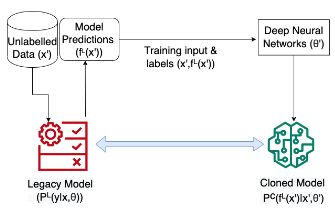
\includegraphics[width=0.5\textwidth]{Example_fig.jpg}
\label{fig:modelclone}
\caption{Example of a figure (Figure 1 from \citealp{aggarwal-zesch-2022-bye}) }
\end{figure}

\begin{table}[htb]
\centering
\caption{Number of issues and papers in \textsc{jlcl} between 2010 and 2015 as an example of formatting a table.}
\label{tab:numberOfPapers}
\begin{tabular}{rrr}
\toprule
year & \#issues  & \#research papers \\
\midrule
2010 & 1 & 5 \\
2011 & 2 & 24 \\
2012 & 2 & 9\\
2013 & 2 & 12\\
2014 & 2 & 11 \\
2015 & 1 & 5 \\
\bottomrule
\end{tabular}
\end{table}






\section{References}

We strongly recommend to use Bib\!\TeX\ to manage references and citations. Bib\!\TeX\  takes care of the correct formatting of the entries in the reference list, but authors are responsible for entering the complete and correct metadata for each reference in the \texttt{.bib}-file.

You can use the \texttt{\textbackslash citep} command to insert author names and year in parentheses in the text. This is an example for citing some papers on various forms of segmentation published in \textsc{jlcl}
\citep{Riedl_Biemann_2012, Jurish_Würzner_2013, Sidarenka_Peldszus_Stede_2015}.
Use the command  \texttt{\textbackslash citet} if the author names are part of the sentence and only the year has to be put in parentheses, e.g.\ if we want to say that \citet{Jurish_Würzner_2013} published a paper in \textsc{jlcl}. If no parentheses should be inserted, the command \texttt{\textbackslash citealp}  can be used.




%https://ctan.math.illinois.edu/macros/latex/contrib/apacite/apacite.pdf

\bibliographystyle{apacite}
\bibliography{references}

\clearpage



\noindent \textbf{Correspondence}

\hspace{12pt}

\noindent Christian Wartena  \orcidlink{0000-0001-5483-1529}\\[0.5\baselineskip]
Hochschule Hannover \\
Data|H Institute for Applied Data Science\\ 
Hannover, Germany\\
\href{mailto: christian.wartena@hs-hannover.de}{christian.wartena@hs-hannover.de}

\end{document}
